\documentclass[12pt]{article}

\usepackage{mathdoc}


%% Numéro de séquence %% Titre de la séquence %%
\renewcommand{\centerhead}{Chap. 2 : Dérivation I}

\begin{document}

\setlength{\parindent}{0cm} 

\section{Limite} %_____________________________

\begin{definition} [Cas général]
Soit f une fonction définie sur un intervalle $]a;b[$ (avec $a<b$).\\
Si, en s'approchant de $c \in ]a;b[$, les valeurs de \( f(x) \) se rapprochent de \( l \), alors on dit que la limite de \( f(x) \) quand \( x \) tend vers \( c \) est \( l \). On écrit : 
\[
\lim\limits_{x \to c} f(x) = l.
\]

\end{definition}

\begin{definition}[Limite en 0]
   On dit qu'une fonction $f$ a pour \underline{limite} $0$ en $0$ si $f(h)$ se rapproche de $0$ dès que $h$ est assez petit.
$$\text{On note :} \quad \lim_{h\to0}f(h)=0$$
\end{definition}
Les fonctions suivantes ont comme limite $0$ en $0$ :
\begin{multicols}{2}
   $\displaystyle{\lim_{h\to0}h=0}$\\
   $\displaystyle{\lim_{h\to0}h^2=0}$\\
   $\displaystyle{\lim_{h\to0}h^3=0}$\\
   $\displaystyle{\lim_{h\to0}\sqrt{h}=0}$
\end{multicols}

\begin{exemple}
   \begin{enuspaced}
      \item $\lim\limits_{h\to0}h+h^2+h^3=0$
      \item $\lim\limits_{h\to0}3h^2-4h=0$
      \item $\lim\limits_{h\to0}-2h^3+\sqrt{h}-1=-1$
   \end{enuspaced}
\end{exemple}


\section{Taux d'accroissement} 

Dans cette partie, $f$ est une fonction numérique définie sur un intervalle $I$, $\mathcal{C}$ sa courbe représentative dans un repère.\\
$a$ et $x$ sont deux réels distincts de $I$.

\begin{definition}
   Le \underline{taux d'accroissement} de la fonction $f$ entre $a$ et $x$ est le quotient :
$$\dfrac{f(x)-f(a)}{x-a}$$
Avec $x=a+h$, ce quotient s'écrit aussi : $$\dfrac{f(a+h)-f(a)}{h}$$
\end{definition}

\begin{exemple}
   Pour $f$ définie sur $\R$ par $f(x)=x^2$, le taux d'accroissement
   de $f$ entre $a$ et $a+h$ est : \\ \\
   \begin{tabular}{p{0.3cm}l!{=}l}
      &  $\dfrac{f(a+h)-f(a)}{h}$ & $\dfrac{(a+h)^2-a^2}{h}$ \\
      & & $\dfrac{a^2+2ah+h^2-a^2}{h}$ \\
      &   $\dfrac{f(a+h)-f(a)}{h}$ & $2a+h$ \\
   \end{tabular}
\end{exemple}

\begin{definition}[Rappel]
La pente d’un segment ou d'une droite, généralement symbolisée par la variable $m$, correspond à la valeur de son inclinaison par rapport à l'axe des abscisses.
\end{definition}

\begin{rappel}
La formule pour calculer la pente $m$ d’une droite qui passe par les
points $A(x_A, y_A)$ et $B(x_B, y_B)$ est : $$m=\dfrac{\Delta
y}{\Delta x} = \dfrac{y_B-y_A}{x_B-x_A}$$
où $\Delta y$ représente la variation des ordonnées et $\Delta x$ représente la variation des abscisses.
\end{rappel}

\begin{remarque}
  Le taux d'accroissement est donc la pente de la droite passant par les points
  $\left(a, f(a)\right)$ et $\left(a+h, f(a+h)\right)$.
\begin{center}
    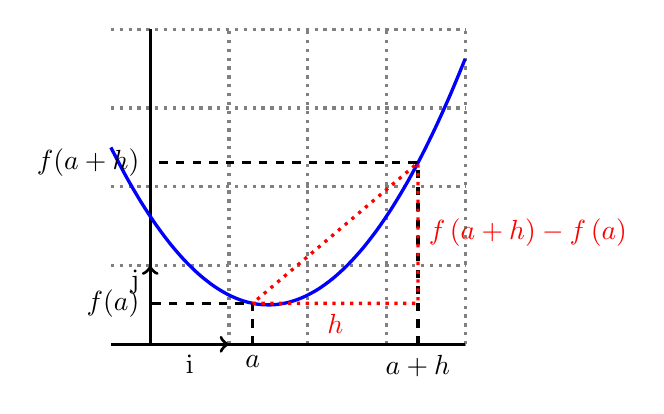
\begin{tikzpicture}[very thick]
      \draw[dotted,color=gray] (-.5,0) grid (4,4);
      \draw[] (-.5,0) -- (4,0);
      \draw[] (0,0) -- (0,4);
      \draw[->] (0,0) -- (1,0) node[midway,below]{i};
      \draw[->] (0,0) -- (0,1) node[midway,above left]{j};
      \draw[domain=-.5:4,smooth,blue] plot ({\x},{pow(\x-1.5, 2)/2+.5});
      \draw[dashed] (1.3, 0) node[below]{$a$} -- ++(0, {pow(1.3-1.5, 2)/2+.5}) -- ++(-1.3, 0) node[left]{$f(a)$};
      \draw[dashed] (3.4, 0) node[below]{$a+h$} -- ++(0, {pow(3.4-1.5, 2)/2+.5}) -- ++(-3.4, 0) node[left]{$f(a+h)$};
      \draw[dotted, red] (1.3, {pow(1.3-1.5, 2)/2+.5}) -- ++({3.4-1.3}, 0) node[below, midway]{$h$} -- (3.4, {pow(3.4-1.5, 2)/2+.5}) node[right, midway]{$f\left( a+h \right)-f\left( a \right)$} -- cycle;
    \end{tikzpicture}
  \end{center}
\end{remarque}

\section{Nombre dérivé} %_____________________________________

\begin{definition}
   On dit que $f$ est \underline{dérivable} en $a$ et on note cette dérivée $f'(a)$ si la limite suivante existe :
$$f'(a)=\lim_{h\to0}\frac{f(a+h)-f(a)}{h}$$
\end{definition}

\begin{remarque}
   On note aussi la dérivée $f'(a)$ comme la limite suivante :
$$f'(a)=\lim_{x\to a}\frac{f(x)-f(a)}{x-a}$$
\end{remarque}

\begin{propriete}[Interprétation géométrique]
  Si une fonction $f$ est dérivable en $a$, alors $f'(a)$ est la pente de la
  tangente à la courbe de $f$ en $(a, f(a))$.
\end{propriete}

\begin{exemple}
  Pour $f$ définie sur $\R$ par $f(x)=x^2$, calculer le nombre dérivé de $f$ en $3$ puis en $-1$ :
   \begin{enumerate}
      \item $\dfrac{f(a+h)-f(a)}{h}=2a+h$ d'après l'exemple $1$
      \item $f'(a)=\lim_{h\to0}2a+h=2a $
      \item $f'(2)=2\times 3=6$
      \item $f'(-1)=2\times (-1)=-2$
   \end{enumerate}
\end{exemple}

\begin{exemple}
On considère la fonction $f$ définie sur $\R$ par $f(x)=x^2+1$.\\
Son taux d'accroissement en $a=1$ est donné par le calcul suivant :
\begin{center}
  \begin{tabular}{p{0.3cm}l!{=}l}
    &  $\dfrac{f(x)-f(a)}{x-a}$ & $\dfrac{(x^2+1)-(1^2+1)}{x-1}$ \\
    & & $\dfrac{(x+1)(x-1)}{x-1}$ \\
    &   $\dfrac{f(x)-f(a)}{x-a}$ & $x+1$ \\
  \end{tabular}
\end{center}
Or, $\lim\limits_{x\to1}x+1=2$\\
Donc $f$ est dérivable en $1$ et $f'(1)=2$
\end{exemple}

\section{Equation de la tangente} %__________________________

\begin{propriete}
   Soit $f$ une fonction numérique définie sur un intervalle $I$ et dérivable en $a\in I$\\
La \underline{tangente} $T_a$ en à la courbe $C_f$ en $a$ a pour équation :
$$T_a : y=f'(a)(x-a)+f(a)$$
\end{propriete}

\begin{demonstration}
\begin{center}
  \begin{tabular}{p{0.3cm}l!{=}l}
    &  $f'(x)$ & $\dfrac{f(x)-f(a)}{x-a}$ \\
    & $f'(x)+\dfrac{f(a)}{x-a}$& $\dfrac{f(x)}{x-a}$ \\
    &   $f(x)$ & $f'(x)(x-a)+\dfrac{f(a)(x-a)}{x-a}$ \\
    &   $f(x)$ & $f'(x)(x-a)+f(a)$ \\
  \end{tabular}
\end{center}
\end{demonstration}

\begin{exemple}
   Soit $f(x)=x^2+2$. Déterminer l'équation de la tangente en $0$ et en $-1$
   \begin{enumerate}
      \item $f'(0)=0$ donc $T_0 : y=0\times(x-0)+f(0)=2$
      \item $f'(-1)=-2$ donc $T_{-1} : y=-2\times(x+1)+f(-1)=-2x+1$
   \end{enumerate}
\end{exemple}

\end{document}
